\documentclass[10pt, conference, compsocconf]{IEEEtran}
%\documentclass[journal,10pt,draftclsnofoot,onecolumn]{IEEEtran}

\usepackage{graphicx,url}
\usepackage{listings}
\usepackage{subfigure}
\usepackage{multirow}
\usepackage[space]{cite}
\usepackage{siunitx}

\sisetup{group-separator = {,}, group-digits = true}
\newcommand\sius[1]{\num[group-separator = {,}]{#1}\si{~\micro\second}}
\newcommand\sims[1]{\num[group-separator = {,}]{#1}\si{~\si{\milli\second}}}
\newcommand\sins[1]{\num[group-separator = {,}]{#1}\si{~\nano\second}}

%\interfootnotelinepenalty=500

\lstset{keywordstyle=\bfseries, flexiblecolumns=true}                           
\lstloadlanguages{[ANSI]C++}
\lstdefinestyle{prg} {basicstyle=\scriptsize, lineskip=-0.2ex, showspaces=false,breaklines=true,showstringspaces=false,numbers=left,numbersep=-7pt,frame=single,stepnumber=1}

\newcommand{\prg}[3][ht!]{
  \begin{figure}[#1]
      \lstinputlisting[language=C++,style=prg,basicstyle=\tiny]{fig/#2.cc}
    \caption{#3\label{prg:#2}}
  \end{figure}
}

\newcommand{\tab}[3][ph]{
  \begin{table}[#1]
    {\centering\small\textsf{\input{fig/#2.tab}}\par}
    \caption{#3}
  \label{tab:#2}
  \end{table}
}

\newcommand{\fig}[4][ht!]{
  \begin{figure}[#1]
    {\centering{\includegraphics[#4]{fig/#2}}\par}
    \caption{#3}
    \label{fig:#2}
  \end{figure}
}

\newcommand{\Fig}[4][hp]{
  \begin{figure*}[#1]
    {\centering{\includegraphics[#4]{fig/#2}}\par}
    \caption{#3}
    \label{fig:#2}
  \end{figure*}
}

\IEEEoverridecommandlockouts

\begin{document}
%
% paper title
% can use linebreaks \\ within to get better formatting as desired
\title{An Experimental Evaluation of the Cache Partitioning Impact\\ on Multicore Real-Time Schedulers~\IEEEauthorrefmark{1}\thanks{\IEEEauthorrefmark{1}This work was supported by the CAPES and DFAIT grants, projects RH-TVD 006/2008 and CAPES-DFAIT 004/11.}}


% author names and affiliations
% use a multiple column layout for up to two different
% affiliations


\author{Giovani Gracioli and Ant\^{o}nio Augusto Fr\"{o}hlich\\
Software/Hardware Integration Lab \\
Federal University of Santa Catarina, Florian\'{o}polis, Brazil \\
\{giovani,guto\}@lisha.ufsc.br
}

% make the title area
\maketitle

\begin{abstract}
Shared cache partitioning is a well-known technique used in multicore real-time systems to isolate task workloads and improve system predictability. Presently, the state-of-the-art studies that evaluate shared cache partitioning on multicore processors lack two key issues. First, the cache partitioning mechanism is typically implemented either in a simulation environment or in a general-purpose OS, and so the impact of kernel activities, such as interrupt handlers and context switching, on the task partitions tend to be overlooked. Second, the evaluation is typically restricted to either a global or partitioned scheduler, thereby by falling to compare the performance of cache partitioning when tasks are scheduled by different schedulers.

In this work, we design and implement a shared cache partitioning mechanism in a multicore component-based RTOS capable of assigning partitions to internal OS data structures, including task and system stacks and interrupt handlers data. We evaluate our shared cache partitioning mechanism running task sets under global (G-EDF) and partitioned (P-EDF) multicore real-time scheduling algorithms. Our results indicate that a lightweight RTOS does not impact real-time tasks, and shared cache partitioning has different behavior depending on the scheduler and the task's working set size.

\end{abstract}

\begin{IEEEkeywords}
shared cache partitioning; real-time operating systems; global scheduling; partitioned scheduling; 
\end{IEEEkeywords}


% For peer review papers, you can put extra information on the cover
% page as needed:
% \ifCLASSOPTIONpeerreview
% \begin{center} \bfseries EDICS Category: 3-BBND \end{center}
% \fi
%
% For peerreview papers, this IEEEtran command inserts a page break and
% creates the second title. It will be ignored for other modes.
\IEEEpeerreviewmaketitle

\section{Introduction}

Current real-time systems are demanding increasing computational power that can only be achieved by the use of multicore processors. However, modern multicore processors have shared resources, such as buses and peripherals, which affect the estimation of the Worst-Case Execution Time (WCET) at the design phase evaluation (schedulability analysis)~\cite{Mancuso:2013}. One of the main factors for unpredictability in multicore processors is the shared cache levels (L2 and L3).

Several recent works have been proposed to deal with shared caches and to provide real-time guarantees. The most common and successful approach is shared cache partitioning~\cite{Liedtke:1997,Kenna:2013}. By assigning separate shared cache partitions to individual tasks, it is possible to isolate task workloads that interfere with one another, leading to increased system predictability. An alternative approach is to use cache partitioning together with a cache locking mechanism, which prevents cache lines from being evicted during program execution~\cite{Suhendra:2008,Sarkar:2012,Mancuso:2013}. The main drawback of cache locking is that it requires specific hardware support that is not present in all commercial processors. 

In general, these recent studies implement and evaluate the proposed approaches either in a simulation environment or in a general-purpose operating system (OS) patched with real-time extensions~\cite{Sarkar:2012,Mancuso:2013,Kenna:2013}. Despite being a good development platform, real-time Linux-based studies suffer from the inherent non real-time behavior of Linux, which interferes with the cache levels (when handling an interrupt, for instance) and may limit the gains obtained by cache partitioning. Also, due to the complexity of the Linux kernel, it is extremely complicated to apply cache partitioning to internal OS data structures and to evaluate the impact of kernel activities, such as interrupt handlers and context switching, which can have a considerable impact on real-time tasks.

Moreover, the scheduling algorithm may also impact the performance gains of a cache partitioning mechanism. In partitioned-based scheduling, tasks are assigned to individual processors and remain on each processor until completing execution. Thus, when a preempted task resumes its execution, part of its data may still be loaded in the same processor's private cache levels. In global-based scheduling tasks are, instead, allowed to migrate among processors during the program execution. Consequently, there is cross-core communication initiated by the cache coherency protocol, which increases the WCET. 

In this paper, we design and implement a cache partitioning mechanism in a component-based RTOS, and compare the cache partitioning behavior using a partitioned and a global scheduling algorithms. Furthermore, our cache partitioning mechanism is able to assign different partitions to the OS, enabling the evaluation of the cache interference impact of the RTOS on hard real-time (HRT) tasks.

In summary, the main contributions of this paper are:

\begin{itemize}
	\item We design and implement an original cache partitioning mechanism in a component-based RTOS, named Embedded Parallel Operating System (EPOS)~\cite{Froehlich:2001,epos}. The mechanism is able to assign partitions to the OS internal data structures and does not rely on any specific hardware support. Additionally, two different approaches are supported that define from which partition data should be allocated: the user-centric approach in which the developer inserts code annotations to define the partition, and the OS-centric approach in which EPOS chooses the partition based on a task ID. 
	
	\item We evaluate the performance of cache partitioning using the Partitioned-EDF and Global-EDF schedulers when both schedulers have total utilization close to the theoretical HRT bounds. Our evaluation is carried out on a modern eight-core processor, with shared Level-3 cache. Our results indicate that cache partitioning has different behavior depending on the scheduler and task's working set size (WSS). We also show an experimental upper-bound in terms of HRT guarantees provided by cache partitioning in each scheduler.
	
	\item By allocating a different cache partition to the internal EPOS data structures, we evaluate the cache interference caused by the RTOS. We show that a lightweight RTOS, such as EPOS, does not impact HRT tasks with separated partitions.
\end{itemize}

The rest of this paper is organized as follow. Section~\ref{sec:back} presents the task model and background concepts. Section~\ref{sec:imp} describes the cache partitioning implementation on EPOS. Section~\ref{sec:eval} presents the evaluation. Main findings are discussed in Section~\ref{sec:disc}. Section~\ref{sec:related} summarizes the related work and Section~\ref{sec:conc} concludes the paper.

\section{System Model and Background}
\label{sec:back}

In this  work, we  consider the periodic task model,  in which a  task set  $\tau$ is composed  of \textit{n}  tasks, \{$T_1,T_2,\ldots,T_n$\}, that are scheduled on \textit{m} identical processors or cores \{$P_{1},P_{2},\ldots,P_{m}$\}. Each task  $T_{i}$, where 1 $\leq$ \textit{i} $\leq$  \textit{n}, has a  period \textit{$p_{i}$} and  a worst-case execution time (WCET) \textit{$e_{i}$}. A task $T_{i}$ releases a job every \textit{$p_{i}$} time units. $r_i^j$ denotes the release time of the $j^{th}$ job of $T_{i}$, named $T_i^j$. The relative deadline of the task $T_i$ is equal to its period: $d_i$ $=$ $p_i$. The fraction \textit{$e_{i}$}/\textit{$p_{i}$} defines the utilization of a task $T_{i}$, called $u_i$. The sum of all tasks' utilizations defines the total system utilization ($\sum_{i=1}^n u_i$).

\subsection{Cache Partitioning and Page Coloring}

Shared cache partitioning is a method to address contention for memory spaces in (real-time) multicore applications. Cache partitioning isolates application workloads that interfere with each other, thus increasing system predictability~\cite{Suhendra:2008}. Cache interference occurs when a preemptive task evicts cache lines from a preempted task, or by kernel activities, such as interrupt handlers, that pollute the shared cache, and when tasks running at the same time on different cores access the same cache line (true or false sharing) and cause inter-core communication.

There are two cache partitioning categories: hardware-~\cite{Qureshi:2006,Suhendra:2008,Shekhar:2012} and software-based~\cite{Liedtke:1997,Chousein:2005,Guan:2009,Muralidhara:2010} techniques. The former requires special hardware support, such as cache locking or specialized implementations, that are not available in most of the current commercial processors. The latter has the advantage of being fully transparent to applications and there is no need for special hardware support.

The most common software-based cache partitioning technique is page coloring~\cite{Liedtke:1997,Tam:2007,Guan:2009}. Page coloring explores the virtual to physical page address translations presented in virtual memory systems at OS-level, when caches are physically-indexed. Page addresses are mapped to pre-defined cache regions, avoiding the overlap of cache spaces. Figure~\ref{fig:bit_field_cache_intel} illustrates the physical addresses from the cache and OS point-of-views for the platform used in our experiments (see Table~\ref{tab:intel-i7}). By controlling the colored bits of the cache associative set number, the OS can change the mapping of 4~KB pages in the physical memory and the cache location. Our platform has an 8~MB shared 16-way set associative L3-cache with 64-bytes per line, and each of the 16 ways can store a cache line. There are $2^{13}$ sets in the cache (8~MB/16ways $\times$ 1way/64~B). Thus, the first 6 bits in the cache address access a cache line, the next 13 bits access a set, and the next 13 bits define a line from one of the 16 ways (Tag in Figure~\ref{fig:bit_field_cache_intel}).

\fig{bit_field_cache_intel}{Physical address view from the cache (on top) and from the OS (bottom).}{width=6.5cm}

The idea of page coloring is to assign color 0 to page 0, color 1 to page 1, and so on, starting again from color 0 after reaching the maximum color number. Figure~\ref{fig:page_organization} shows the mapping of physical pages to cache locations in our platform. There are 64 cache lines in each 4~KB page. Each of these lines has a different cache set index. Since 7 bits are available to page coloring (cache size / number of ways / page size), page 128 maps to the same color as page 0. It is possible to partition the cache by assigning different colors to tasks.

\fig{page_organization}{Mapping physical pages to cache locations.}{scale=.45}

Cache partitioning and page coloring can still have cache lines evicted due to non-predictable cache line replacement policies (intra-task interference) or by non-colored kernel pages. Although important, we do not focus on the cache replacement issues in this work. Our proposed page coloring based cache partitioning allows the partitioning of both kernel and application data.

\subsection{Global and Partitioned Real-Time Schedulers}

Real-time schedulers are classified in two categories: global and partitioned~\cite{Carpenter2004}. In a global scheduler, there is only one ready queue, where a pre-defined scheduling criterion orders the jobs accordingly. The scheduler assigns a job to any of the available processors. A migration occurs when a job is preempted and later resumed in another processor. In a partitioned scheduler, a partitioning heuristic statically assigns tasks into available processors. Then, each partition executes the scheduling separately~\cite{Liu:2000}. Consequently, there are no job migrations.

Global Earliest-Deadline-First (G-EDF) and Partitioned-EDF (P-EDF) are examples of each category. Although suboptimal, G-EDF has less frequent preemptions and migrations, and consequently less run-time overhead, than optimal global schedulers~\cite{Brandenburg:2008}, such as PFair-based schedulers~\cite{Baruah96,Levin:2010}. Furthermore, optimal multicore real-time schedulers are difficult to implement in practice, and G-EDF has reasonable run-time overhead for a moderate number of processors~\cite{Bastoni:2010}. Also, G-EDF is interesting for mixed-criticality systems, where applications with different criticality levels co-exist in the same system, because it ensures tardiness bounds for soft-real time (SRT) applications as long as the total system utilization is at most \textit{m}, where \textit{m} is the number of processors~\cite{Leontyev:2007}. P-EDF, on the other hand, has a limitation due to similarity to the bin-packing problem: heavy utilization tasks\footnote{A task that has a utilization higher than 0.5 is considered a heavy task.} strongly affect task partitioning heuristics. P-EDF is superior to G-EDF for HRT scenarios~\cite{Gracioli:2013}. In our experimental evaluation, we use both G-EDF and P-EDF.

\section{Implementation Description}
\label{sec:imp}

We implemented our page coloring based cache partitioning in the Embedded Parallel Operating System (EPOS)~\cite{Froehlich:2001,epos}. EPOS is a multi-platform, object-oriented, component-based, embedded system framework implemented in C++. Platform-independent system components implement traditional OS services, such as threads and semaphores. Hardware mediators implement platform-specific support~\cite{Polpeta2004}. Hardware mediators are functionally equivalent to device drivers in Unix, but do not build a traditional Hardware Abstraction Layer (HAL). Instead, hardware mediators sustain the interface contract between software and hardware by means of static metaprogramming techniques and inlining code that ``dilute'' mediator code into components at compile time (no calls, no layers, no messages; mostly embedded assembly). In the next subsections, we summarize the real-time and memory management support on EPOS and the page coloring implementation carried out by this work.

\subsection{Multicore Real-Time Support on EPOS}
\label{sec:epos_real_time}

EPOS implements several real-time schedulers, including G-EDF and P-EDF~\cite{Gracioli:2013}. A \texttt{Periodic\_Thread} class represents a real-time task, aggregating mechanisms related to the periodic task re-execution. The class has a semaphore that is called by the \texttt{wait\_next} method to put a thread to sleep until the next period (traditional \texttt{p} operation of a semaphore). When a timer interrupt arrives, the timer handler (an \texttt{Alarm}) performs a \texttt{v} operation on the semaphore to release and wake-up the task. 

Figure~\ref{fig:uml_sequence_thread_wakeup} depicts the UML sequence diagram of the wake-up operation. The \textbf{alt} label represents an if/else condition and the \textbf{opt} label represents an if clause. The \texttt{begin\_atomic} method protects shared data by locking a \texttt{spinlock} and disabling interrupts. The thread \texttt{reschedule} method releases the \texttt{spinlock} and enables interrupts. The \texttt{Semaphore} calls the \texttt{wakeup} method, which removes the \texttt{Thread} blocked on the semaphore's \texttt{Queue} and calls the scheduler to reinsert the thread into the scheduler list (\texttt{resume} method) according to the defined scheduling criterion (EDF or RM for instance). If the scheduling criterion is dynamic (like the EDF), the priority of the releasing thread is recalculated. In the end, the \texttt{wakeup} method calls the thread \texttt{reschedule} to choose the highest priority task to be executed (see~\cite{Gracioli:2013} for a complete overview on EPOS multicore real-time support).

\fig{uml_sequence_thread_wakeup}{UML sequence diagram of thread wake-up method.}{scale=.45}


\subsection{Memory Management on EPOS}

Portable OSes face a challenge in terms of memory management: some computing platforms feature sophisticated MMUs, while other platforms do not provide any support to map and protect address spaces. The EPOS' careful design encapsulates details pertaining to address space protection, translation, and physical memory allocation into the MMU hardware mediators, which allows memory management components to be highly portable across virtually any platform, from simple microcontrollers to complex multicore processors~\cite{Polpeta2004}.

Figure~\ref{fig:uml_class_mmu} shows part of the MMU mediators family. The \texttt{MMU\_Common} parameterized class provides basic functions common to all architectures. Different classes specialize the base class, implementing architecture-dependent functions. The \texttt{IA32\_MMU} class implements the support for the 32-bit paging mode available on x86 processors, including the manipulation of page and directory tables. A grouping list organizes the available physical memory. Each list element represents a free physical memory space. The MMU initialization method initializes the grouping list according to the available memory.

\fig{uml_class_mmu}{IA32 MMU hardware mediator.}{scale=.4}

Figure~\ref{fig:uml_class_as_seg} depicts the system components that deliver the main available memory to applications. A \texttt{Segment} is a chunk of memory that stores arbitrary code and data. When a system component creates a \texttt{Segment}, the \texttt{MMU::Chunk} inner class allocates the requested memory size from the MMU grouping list and maps the allocated pages to corresponding page table entries. The \texttt{Address\_Space} component is a container for memory chunks (\textit{e.g.}, \texttt{Segments}), that manages the physical memory corresponding to a memory segment, thus keeping the \texttt{Segment} independent of a memory management policy. When a \texttt{Segment} is attached to an \texttt{Address\_Space}, the \texttt{Address\_Space} maps all previously allocated page tables to corresponding page directories through the \texttt{MMU::Directory} inner class.

\fig{uml_class_as_seg}{UML class diagram for address space and segment components.}{scale=.4}

Applications do not allocate memory directly from the \texttt{Address\_Space} and \texttt{Segment} components. Instead, two different heap class instances, which use the described memory management components, provide free memory for the OS and applications. Dynamic memory allocations from the OS, such as creation of thread stacks and system objects, go to the system heap, while requests from the application go to the application heap. During the EPOS initialization, each heap frees its pre-defined (configurable) size by using the \texttt{Address\_Space} and \texttt{Segment} components, as demonstrated in the next subsection.

\subsection{Colored Memory Allocation}

To support page coloring in EPOS, we changed the memory management system components, the MMU hardware mediator, and heap initialization. Figure ~\ref{prg:mmu_traits} shows the new MMU trait class\footnote{A trait class is a template class that associates information of a component at compile time.} that enables page coloring in the system.

\prg{mmu_traits}{IA32 MMU trait class responsible for enabling page coloring.}

When the developer enables page coloring, the MMU grouping list becomes an array of \textit{N} grouping lists and the application heap becomes an array of \textit{N}  heaps, where \textit{N} is the number of colors defined in the trait class. If the defined number of colors is less than the maximum number of colors, then the colors are grouped, forming a \textit{super color}\footnote{We use color to refer to super color hereafter.}~\cite{Lin:2008}: 

\begin{equation}
Super\ color = page\ color\ \%\ max.\ num.\ of\ colors
\end{equation}

The MMU mediator fills each grouping list with pages associated with the corresponding color at the initialization phase. In the same way, the \texttt{Segment} component provides, in its interface, a way to specify from which color (\textit{i.e.}, from which MMU grouping list) a heap should allocate memory. Since each MMU grouping list has a set of physically mapped pages, with the same color, we make sure that each heap has a chunk of logical addresses that map to physical pages with the same color.

Figure~\ref{fig:uml_sequence_heap_init} exemplifies the application heap initialization. The init process creates, for each color, a \texttt{Segment} with the heap size and attaches this \texttt{Segment} to an \texttt{Address\_Space}. The \texttt{free} method receives the logical address returned by the \texttt{attach} method, and then initializes the heap free space.  Moreover, the \texttt{set\_color} method sets the heap color. To properly release a memory space, we use the defined color to find from which heap a memory address was allocated, as will be explained in the next subsection. We initialize the system heap in the same way, but we always allocate the memory for the system heap from the same MMU grouping list (only one \textit{super color}). It is possible to include several system heaps with different colors as well, but this would require changes in the source code of the system components to define the appropriate color. Since our objective is to analyze possible interference between OS and applications, only one system heap is enough. Below, we propose two different approaches to specify the heap for a dynamic allocation: user-centric and OS-centric.

\fig{uml_sequence_heap_init}{UML sequence diagram of the colored application heap initialization.}{scale=.45}

\subsection{User-Centric Approach}

The C++ \texttt{new} and \texttt{delete} operators perform the dynamic memory allocation operations. We overload the EPOS \texttt{new} operator to include annotations (\textit{i.e.}, colors) that define from which heap data should be allocated. Figure~\ref{prg:operator_new} shows how the \texttt{new} and \texttt{delete} operators use these annotations. An enumeration defines the available colors. We changed the \texttt{new} operator to receive, in addition to the requested number of bytes, the color number. If the application does not specify a color, the \texttt{new} operator uses the color 0. Additionally, the \texttt{new} operator prints a message and does not allocate memory if the requested color is greater than the maximum color, defined in the trait class (see Figure~\ref{prg:mmu_traits}).

\prg{operator_new}{Overload of the EPOS \texttt{new} operator.}

The heap allocates eight bytes (two integers) more than the requested size: the first integer contains the data size (the \textit{bytes} argument) and the second integer contains the color number. Thus, the \texttt{delete} operator releases the allocated memory using the correct heap and size by reading the two integers. The overload of the \texttt{new} operator is part of the ISO C++ standard and, is supported by any standard C++ compiler. Figure~\ref{prg:mmu_traits} shows the MMU trait class that defines the use of the user-centric approach.

\subsection{OS-Centric Approach}

When the developer enables the OS-centric approach, the \texttt{new} operator ignores the annotated color (there is no need to pass a color). EPOS transparently chooses from which heap data should be allocated by using a thread ID to access a colored heap: ID \% Traits$<$MMU$>$::colors. It is important to highlight that the choice of either user-centric or OS-centric is made at compile time, without any run-time overhead. The thread constructor assigns a unique ID to each thread; however, in this approach, the user should properly define the number of colors to avoid allocations from the same heap, giving consideration to the number of threads in the target application. The choice of the best number of colors for an application is not straightforward, because it depends on the WSS of each task and how each task uses its own WSS. The objective of this work is to empirically evaluate the impact of cache partitioning on multicore real-time schedulers, and not to optimize the number of colors.

\section{Experimental Evaluation}
\label{sec:eval}

In this section, we discuss the experiments with generated task sets. We execute all experiments on an Intel i7-2600 processor (see Table~\ref{tab:intel-i7}). We set the number of super colors according to the number of tasks in a task set, plus two additional colors: one for an uncolored heap and another one for the OS. For instance, in a task set with ten tasks, we set the number of colors to twelve. We focus on HRT systems, where deadlines must be always met.

\begin{table}[htb]
\begin{center}
\caption{Intel i7-2600 processor features.}
\tiny{
\begin{tabular}{|c|c|}
\hline
Clock speed & 3.4~Ghz\\
\hline
Cores & 4\\
\hline
SMT (hyperthreading) & 2 per core (8 logical cores)\\
\hline
L1 cache & 4 x 64~KB 8-way set associative (32~KB \\
         & separate data and instructions caches)\\
\hline
L2 cache (non-inclusive) & 4 x 256~KB 8-way set associative (unified)\\
\hline
L3 cache (inclusive) & 8~MB 16-way set associative (unified)\\
\hline
\end{tabular}
}
\label{tab:intel-i7}
\end{center}
\end{table}

\subsection{Task Sets Generation and Experiment Description}
\label{sec:task_generation}

We randomly generated task sets similar to~\cite{Kenna:2013}. We selected the periods (all values are in~\si{\milli\second}) uniformly from \{25, 50, 100, 200\} and utilizations uniformly between [0.1, 0.7]. The WCET of a task is defined according to the generated period and utilization. For G-EDF, we generated tasks in a task set until the GFB schedulability test fails~\cite{Goossens:2003}. For P-EDF, we generated tasks in a task set until the best-bit partitioning heuristic fails. P-EDF usually has a better system utilization for HRT than G-EDF, and thus will have a few more tasks in the task sets~\cite{Gracioli:2013}. The objective is to evaluate the performance of G-EDF and P-EDF when both schedulers are close to theoretical HRT bounds. We generated ten task sets for each scheduler.

Each task executes a function that allocates its WSS, reading and writing to the WSS (an array), in a loop, randomly. Figure~\ref{prg:app} shows part of the function source code. We considered scenarios with different WSS: 32~KB, 64~KB, 128~KB, and 256~KB. We defined a write ratio of 25\% (one write in a cache line after four readings). The number of reads and writes of a task varies depending on the WCET. We ran a task in an unloaded system and associated the obtained WCET to the WCET of the other tasks (the repetitions parameter in Figure~\ref{prg:app}). We executed some experiments following this methodology, and ensured that the WCET of each task was never greater than the generated WCET. With this approach, time is made available for OS overhead (scheduling, context switching, release, IPI latency, and tick counting)~\cite{Gracioli:2013}. Thus, the total utilization of the task sets remains close to the generated utilization. We did not use a tool to automatically extract the WCET, because there is no tool for our processor due to its complexity.

\begin{figure}[!ht]
\lstset{language=C++,style=prg,basicstyle=\tiny}
\begin{lstlisting}
    #define ITERATIONS 200
    #define MEMORY_ACCESS 16384
    #define WRITE_RATIO 4
    static bool same_color = false;
    int job(unsigned int repetitions, int id)
    {
      int sum = 0;
      Pseudo_Random * rand;
      int *array;
      if(same_color) {
          rand = new (COLOR_2) Pseudo_Random();
          array = new (COLOR_2) int[ARRAY_SIZE];
      } else {
          rand = new (id+2) Pseudo_Random();
          array = new (id+2) int[ARRAY_SIZE];
      }
      rand->seed(clock.now() + id);
      for(int i = 0; i <  ITERATIONS; i++) {
          Periodic_Thread::wait_next();
          for(int j = 0; j < repetitions; j++) {
              for(int k = 0; k < MEMORY_ACCESS; k++) {
                  int pos = rand->random() % (ARRAY_SIZE - 1);
                  sum += array[pos];
                  if((i % WRITE_RATIO) == 0)
                      array[pos] = k + j;
              }
          }
       }
    }
\end{lstlisting}
\caption{Part of the task function source code.}
\label{prg:app}
\end{figure}

The lowest priority task in a task set executes a function that reads from and writes to an array of 512~KB in a loop, emulating a periodic server that executes best-effort tasks. We choose a WSS of 512~KB, because when allocating the memory sequentially in this size, the task reads and writes using all cache lines (128 pages). We randomly choose the array position of the first read at the beginning of each period, and increment each reading and writing by 64 (cache line size) per loop iteration. All tasks repeat for 200 periods, which results in a total execution time of about 40~\si{\second}.

\subsection{Evaluation on the Individual Task Execution Time}

To evaluate the different page coloring allocation mechanisms and the influence of the OS on the WCET of tasks, we considered three different memory allocation scenarios:

\begin{itemize}
	\item \textbf{S1:} EPOS and each task allocate data from a different super color, as described in Section 3.
	\item \textbf{S2:} Each task allocates data from a different super color. EPOS allocates data from a non-colored and sequential heap. This creates interference between data allocated by EPOS and the data of each task, because EPOS can access a cache line of any color.
	\item \textbf{S3:} Each task allocates data from the same super color. EPOS allocates data from a different super color.
\end{itemize}

All tasks in the third scenario designedly allocates memory from the same super color, possibly sharing the same cache lines, reflecting a worst-case scenario. As explained in~\cite{Kenna:2013}, safety-critical applications have security requirements in which the prevention of malicious tasks that evict cache lines from other tasks is desirable. The second scenario evaluates the interference of EPOS with the periodic tasks. Figure~\ref{prg:app} shows the scenarios S1 and S3 (the \texttt{same\_color} boolean variable, lines 10 to 16). For the second scenario, we changed the MMU initialization to construct a grouping list without any color (\textit{i.e.,} sequential addresses) and then, the system heap allocates memory from this grouping list.

We executed the ten different task sets of G-EDF and P-EDF in each scenario for 50 times, varying the WSS as described in the previous Section (more than 66 hours of tests using a real hardware and an RTOS). Then, we extracted the WCET and AVG execution time of each task for each scenario and WSS from these executions. We calculate the WCET scaling factor, $x_i^j$ / ($WCET_i^j$ in $S1$), where $i$ is a task in the task set $j$, and $x$ is the obtained WCET of $T_i$. Thus, $x_i^j$ represents the WCET of $T_i$ executing in either S2 or S3, divided by the obtained WCET for the same task $T_i$ executing in S1. We do the same for the AVG scaling factor: $y_i^j$ / ($AVG_i^j$ of $S1$), where $y_i^j$ represents the obtained AVG execution time of $T_i$ executing in either S2 or S3 and $AVG_i^j$ represents the AVG execution time of $T_i$ in S1. The AVG scaling factor is interesting for providing SRT guarantees. 

We then calculate the average WCET and AVG scaling factors of each task set, varying the WSS. Figure~\ref{fig:sca_worst_case} presents the obtained WCET scaling factors and Figure~\ref{fig:sca_average} shows the results for the AVG scaling factors. On the x-axis, we vary the WSS and, on the y-axis, we show the obtained scaling factors. Note that the scaling factors for S2 are equal to one, meaning that when EPOS uses an uncolored heap, it does not affect the tasks' execution time. EPOS interrupt service routines (ISRs) have a small fingerprint and use few bytes, generating very small interference on cache lines. Additionally, for 32 and 64~KB, the WCET scaling factor for the G-EDF is greater than that P-EDF. As two logical cores share the same L2-cache with 128~KB, the contention for cache lines is more frequent and there are more inter-core communication (bus snooping caused by the cache coherency protocol). When setting a WSS to 32~KB, all data is possibly loaded to the L2-cache. When the WSS is 64~KB, the scaling factor increases due to higher number of misses on the L1-cache in S3 and the similar obtained WCET in S1 due to tasks isolation. When the WSS is 128 and 256~KB, the delay caused by the intra-task cache misses increases the AVG and WCET of tasks, thus decreasing the scaling factors. Also, for WSSs of 128 and 256~KB, P-EDF has a greater WCET scaling factor due to the contention caused by two tasks running on the same logical core, sharing the L1 and L2-caches. In the next Section, we correlate the obtained scaling factors with deadline misses.


\begin{figure}[htb]
\centering
\subfigure[] {
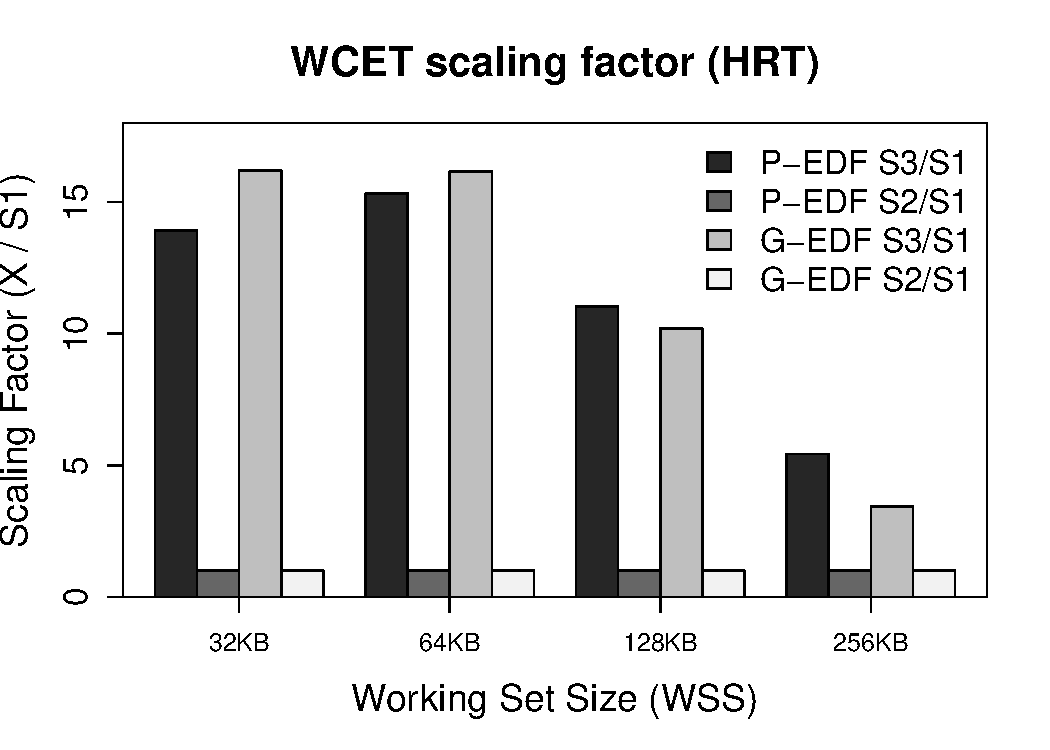
\includegraphics[scale=.37]{fig/worst_case_ind_exec_time}
\label{fig:sca_worst_case}
}
\subfigure[] {
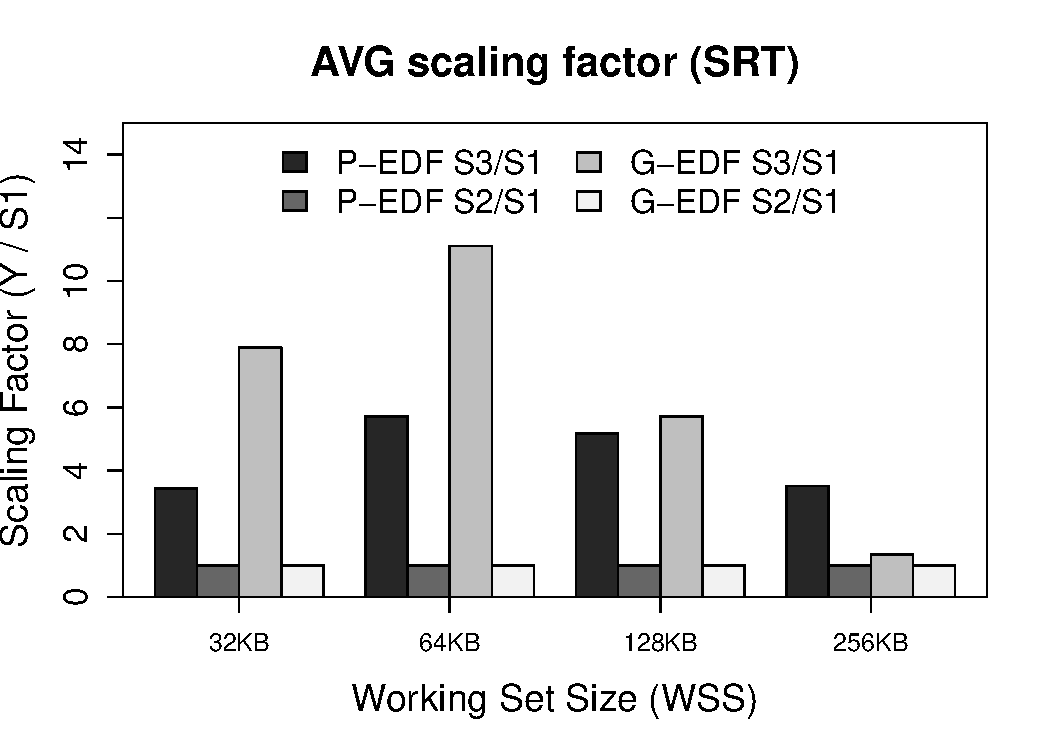
\includegraphics[scale=.37]{fig/avg_case_ind_exec_time}
\label{fig:sca_average}
}
\caption{(a) Obtained worst-case scaling factors (hard real-time). (b) Obtained average scaling factors (soft real-time).}
\label{fig:scaling_factor}
\end{figure}

\subsection{Deadline Misses and Total Execution Time}

%Figure~\ref{fig:scaling_factor} has shown a WCET scaling factor of up to 15.32 times (G-EDF and WSS of 64~KB). 
Figure~\ref{fig:percentage_of_missed_deadlines} presents the percentage of tasks that missed their deadlines, in all task sets and varying the WSS. The x-axis presents the WSS and the y-axis the percentage of tasks that missed their deadlines. We do not show the S2, because it has the same behavior of S1. Our focus here is on HRT, consequently we show the percentage of all tasks that missed at least one deadline and not the total number of missed deadlines per task. For WSS of 32 and 64~KB, both P-EDF and G-EDF in S1 do not miss any deadline. About 18\% of tasks in G-EDF executing in S1 with 128~KB missed deadlines. This is mainly due to the cache contention caused by the MESIF cache coherency protocol. When a task is preempted and migrates to another core, it reloads the data that was on the original core. Thus, the cache controller causes invalidation on the cache lines used by the preempted task. The cost of an invalidation is comparable to access the main memory~\cite{intelopt}. For P-EDF in S3, the percentage of tasks that missed deadline was 57.75\%, 70.42\%, 74.65\%, and 93.02\%, for 32, 64, 128, and 256~KB, respectively. For G-EDF in S3, the percentage was 93\%, 93.02\%, 93.92\%, and 97.67\%. For 256~KB in S1, 54.93\% and 92\% of tasks missed their deadline in P-EDF and G-EDF, respectively. We can conclude that cache partitioning provides safe HRT bounds for WSSs of 32 and 64~KB for both G-EDF and P-EDF, and for WSS of 128~KB for P-EDF. 

\fig{percentage_of_missed_deadlines}{Percentage of tasks that missed their deadline when varying the data size and using the P-EDF and G-EDF schedulers in S1 and S3.}{scale=.37}

Figure~\ref{fig:total_exec_time} shows the total obtained application execution time for S1 and S3 (\textit{i.e.,} the total time to finish all tasks in a task set). Again, we do not show S2, because it has the same performance of S1. The x-axis shows the WSS and the y-axis the total execution time in seconds. As described in Section~\ref{sec:task_generation}, each task iterates for 200 times, and the greatest possible period for a task is 200~\si{\milli\second}, which gives us an expected execution time of 40~\si{\second} (all task sets have at least one task with a period of 200~\si{\milli\second}). This Figure can be correlated to Figure~\ref{fig:percentage_of_missed_deadlines} in terms of the frequency of deadline misses. For example, for WSS of 32~KB and S3 and G-EDF scheduler, 93\% of tasks lost at least one deadline; however, we can see that total execution time is still 40~\si{\second}. This suggests that the occurrence of deadline misses is infrequent. As the WSS increases, the total application time also increases; tasks miss their deadlines more frequently, and constantly overrun their periods. There is no handling mechanism for tasks that overrun their periods. As described in Section~\ref{sec:epos_real_time}, the \texttt{Alarm} component releases a task with a \texttt{v} operation on a semaphore and the task waits for the next period by calling the \texttt{p} operation. When a task overrun its periods, the \texttt{p} operation found the semaphore with a value greater than one, and does not put the task to sleep. Instead, the \texttt{v} operation returns immediately and the task keeps executing. For WSS of 128~KB in S1 with G-EDF, 18\% of tasks lost their deadlines; however, the total application time is 40~\si{\second}. When the system is overloaded (256~KB), G-EDF is able to handle the tasks more efficiently: a waiting task can execute as soon as a core is available. 

\fig{total_exec_time}{Total application execution time when varying the data size and P-EDF and G-EDF with and without page coloring.}{scale=.37}

\section{Discussion}
\label{sec:disc}

Below, we summarize our main findings:

\begin{itemize}
	\item \textbf{Cache hierarchy effects:} cache partitioning isolates task workloads and provide predictability for multicore real-time systems in terms of memory hierarchy perspective. For P-EDF, page coloring supported up to 128~KB, and for G-EDF up to 64~KB. To support larger WSSs, cache partitioning could be used together with hardware techniques, such as cache locking. Even when tasks miss their deadlines with cache partitioning (128~KB for G-EDF, and 256~KB for P-EDF and G-EDF), the advantage is predictability of cache accesses. It is possible to apply a data reuse method~\cite{Jiang:2010} and provide HRT guarantees during the theoretical schedulability analyses.

	\item \textbf{P-EDF and G-EDF behaviors:} cache partitioning was more efficient in G-EDF for WSSs up to 64~KB, by helping to prevent inter-core communication through the cache coherency protocol. All data is able to fit in L2-cache and the invalidations in the L3-cache are reduced when compared to S3. For 128 and 256~KB, page coloring was more efficient in P-EDF, because cache partitioning reduces contention for cache spaces when tasks are running on two logical cores at the same time. Moreover, in an underloaded system, G-EDF handles the tasks more efficiently than P-EDF, because tasks can migrate as soon as a core becomes available. As the WSS increases, there is more intra-task interference (cache misses in the same cache partitions), which increases the task execution time in S1 and reduces the scaling factor. Inter-core communication, caused by task migrations, has a considerable impact on HRT tasks (18\% of missed deadlines), as shown in G-EDF with WSS of 128~KB.
	
	\item \textbf{Shared data among tasks:} when tasks execute in parallel on different cores and share data, they will access the same cache lines, causing invalidations handled by a bus snooping protocol. Cache partitioning does not solve the problem, but it helps to keep all data organized in memory. Providing a separate set of colors to shared data may improve the overall performance~\cite{Chen:2009}. Moreover, a shared-data-aware real-time scheduler can reduce the access serialization to the same cache line and saturation in the inter-core interconnection by avoiding the scheduling of tasks with shared data at the same time.
	
	\item \textbf{Exclusive color for the RTOS:} EPOS is a lightweight RTOS. ISRs and scheduling operations in EPOS have a small footprint and use few bytes. Consequently, using an exclusive color for EPOS did not make any difference. ISRs of network and disk devices usually have large buffers and may benefit from having an exclusive color. Our page coloring mechanism is able to provide exclusive colors for different ISRs.
	
	%\item Pessimistic iterations: we consider that threads always execute for the WCET. This may not be true for all applications. An extension is to incorporate a distribution method to define the number of repetitions during a period. 
	
	\item \textbf{RTOS and general-purpose OS}: related work on cache partitioning and real-time systems usually use real-time patches applied to a general-purpose OS, such as Linux. Our evaluation was entirely carried out using a RTOS and real hardware. We believe that with the page coloring support implemented in this work, EPOS has improved its real-time support and temporal isolation among real-time tasks, providing a better multicore real-time open source research platform.
	
	\item \textbf{Cache coherency protocols and memory architectures}: we used a processor with ccNUMA memory architecture in our experiments. Usually, ccNUMA processors use MESIF or MOESI cache-coherence protocols, while UMA architectures use MESI protocol. The processor interconnect between these two architectures presents considerable differences. For example, the Intel's Quickpath Interconnect (QPI) provides higher bandwidth and lower latency for NUMA-based architectures than the Front-Side Bus (FSB), typically used in UMA architectures. Each processor has an integrated memory controller and features a point-to-point link, allowing parallel data transfer and shortest snoop request completion. In consequence, ccNUMA-based processors have a faster communication among cores. Thus, cache partitioning on UMA-based processors should be even more efficient. 
\end{itemize}

\section{Related Work}
\label{sec:related}

Several shared cache partitioning mechanisms for general-purpose systems have been proposed recently~\cite{Lin:2008,Chen:2009,Muralidhara:2010}. Usually, such mechanisms aim at reducing the last-level cache misses, and thus increasing the QoS and fairness. Most of the proposed approaches are software-based, using the page coloring method~\cite{Lin:2008,Chen:2009} or specific user-level APIs~\cite{Ding:2011}, while other approaches proposed some special hardware support~\cite{Qureshi:2006,Suhendra:2008}. Our page coloring based cache partitioning allows the memory to be transparently allocated by the OS or performed by the developer using specific code annotations, as demonstrated in Section~\ref{sec:imp}.

Shared cache partitioning has also been used to increase the predictability of real-time systems~\cite{Liedtke:1997,Chousein:2005,Guan:2009}. Compiler-based techniques partition the shared cache space by accessing the source code and allocating partitions to tasks at compile time~\cite{Vera:2003}. Cache locking prevents the eviction of cache lines during the program execution~\cite{Aparicio:2012,Sarkar:2012}. Cache locking is a hardware specific feature and, although useful to increase the system predictability, it is not present in all of the today's commercial processors. Cache locking has been used to provide more predictability for migration tasks under global and semi-partitioned schedulers~\cite{Sarkar:2011,Shekhar:2012}.

$MC^2$ treats the management of cache lines as synchronization and scheduling problems~\cite{Kenna:2013}. The proposed approach uses page coloring and real-time multiprocessor locking protocols together. The OS associates a set of colors to each task. Then, a task locks its set of colors whenever it is invoked or portions of cache are viewed as preemptive resources that are scheduled. The authors compared both techniques in terms of schedulability of the P-RM algorithm and concluded that cache locking approach is better than the scheduling approach. In our work, we extended the page coloring performance analysis to P-EDF and G-EDF algorithms and considered also the impact of the OS on the WCET. Unlike $MC^2$, which is implemented using a real-time patch for Linux, we evaluated the cache partitioning and the real-time algorithms on an RTOS designed from scratch, with less interference~\cite{Gracioli:2013}. Mancuso \textit{et al.} proposes a memory framework that uses profiling techniques to analyze the memory access pattern of tasks and obtain the most frequently accessed memory pages~\cite{Mancuso:2013}. Then, cache locking and page coloring are used to provide isolation among tasks and increase predictability. This work also used Linux and requires hardware with cache locking support.	

Other approaches change the OS memory allocator to be cache-aware. Chilimbi \textit{et al.} proposed a memory allocator that receives the requested bytes and a pointer to an existing data object~\cite{Chilimbi:2000}. The objective is to allocate the requested data block next to the existing data block, and thus improving data locality, cache hit rates, and the average execution time. Cache-Aware Memory Allocator (CAMA) receives allocation requests with a cache set as an additional parameter~\cite{Herter:2011}. The allocator keeps different free memory lists organized by cache sets, similar to our approach. Also, CAMA guarantees to access only a known subset of the available cache sets in a bounded time. Our memory allocation mechanism has the advantage of being non-intrusive (there is no need to create a new function as in CAMA) and to support user- and OS-centric approaches.
%Cache-index also tries to improve the average execution time, instead of improving the predictability~\cite{Afek:2011}. 

\section{Conclusion}
\label{sec:conc}

Shared cache memory partitioning is an efficient approach to increase predictability of multicore real-time systems. In this work, we have designed and implemented a cache partitioning mechanism based on page coloring in a component-based RTOS. We have evaluated the gains of cache partitioning using two different multicore real-time scheduling algorithms (P-EDF and G-EDF) in a modern eight-core processor with shared L3-cache. We have also evaluated the cache interference impact of the RTOS on HRT tasks by assigning individual colors to the internal RTOS data structures. A lightweight RTOS does not have a considerable cache interference for HRT tasks. The results have also shown that cache partitioning provide more gains for G-EDF when tasks' WSSs are up to 64~KB, while for WSS of 128 and 256~KB, it provides a better workload isolation for P-EDF. Furthermore, in an underloaded system, G-EDF handles the tasks more efficiently than P-EDF, because tasks can migrate as soon as a core becomes available.

As future work, we plan to apply our page coloring mechanism in a distributed H.264 motion estimation algorithm, port EPOS to a multicore ARM processor, and to investigate how a shared-data-aware real-time scheduler can use page coloring and hardware performance counters to provide real-time guarantees for parallel real-time tasks with shared data.

% conference papers do not normally have an appendix

% trigger a \newpage just before the given reference
% number - used to balance the columns on the last page
% adjust value as needed - may need to be readjusted if
% the document is modified later
%\IEEEtriggeratref{8}
% The "triggered" command can be changed if desired:
%\IEEEtriggercmd{\enlargethispage{-5in}}

% references section

\bibliographystyle{IEEEtran}
\bibliography{references}

% that's all folks
\end{document}


